\documentclass[10.5pt,]{article}

\usepackage{multicol} % for multiple columns



\usepackage[sc, osf]{mathpazo}
\usepackage{amssymb,amsmath}
\usepackage{ifxetex,ifluatex}
\usepackage{fixltx2e} % provides \textsubscript
\ifnum 0\ifxetex 1\fi\ifluatex 1\fi=0 % if pdftex
\usepackage[T1]{fontenc}
\usepackage[utf8]{inputenc}
\else % if luatex or xelatex
\ifxetex
\usepackage{xltxtra,xunicode} %originally, \usepackage{mathspec}. This change is to produce Chinese
\else
\usepackage{fontspec}
\fi
\defaultfontfeatures{Ligatures=TeX,Scale=MatchLowercase}
\fi
% use upquote if available, for straight quotes in verbatim environments
\IfFileExists{upquote.sty}{\usepackage{upquote}}{}
% use microtype if available
\IfFileExists{microtype.sty}{%
	\usepackage{microtype}
	\UseMicrotypeSet[protrusion]{basicmath} % disable protrusion for tt fonts
}{}
\usepackage[margin=1in]{geometry}




\setlength{\emergencystretch}{3em}  % prevent overfull lines
\providecommand{\tightlist}{%
	\setlength{\itemsep}{0pt}\setlength{\parskip}{0pt}}
\setcounter{secnumdepth}{0}
% Redefines (sub)paragraphs to behave more like sections
\ifx\paragraph\undefined\else
\let\oldparagraph\paragraph
\renewcommand{\paragraph}[1]{\oldparagraph{#1}\mbox{}}
\fi
\ifx\subparagraph\undefined\else
\let\oldsubparagraph\subparagraph
\renewcommand{\subparagraph}[1]{\oldsubparagraph{#1}\mbox{}}
\fi

% Now begins the stuff that I added.
% ----------------------------------

% Custom section fonts
\usepackage{sectsty}
\sectionfont{\rmfamily\mdseries\large\bf}
\subsectionfont{\rmfamily\mdseries\normalsize\itshape}


% Make lists without bullets
\renewenvironment{itemize}{
	\begin{list}{}{
			\setlength{\leftmargin}{1.5em}
		}
	}{
	\end{list}
}


% Make parskips rather than indent with lists.
\usepackage{parskip}
\usepackage{titlesec}

\usepackage{ctex}
% Siyuan Font
%\setCJKmainfont[BoldFont = Noto Sans CJK SC]{Noto Serif CJK SC}
%\setCJKsansfont{Noto Sans CJK SC}
%\setCJKfamilyfont{zhsong}{Noto Serif CJK SC}
%\setCJKfamilyfont{zhhei}{Noto Sans CJK SC}
%\setCJKfamilyfont{zhkai}{simkai.ttf}

% less space for the Chinese format
\titlespacing\section{0pt}{1pt plus 4pt minus 2pt}{1pt plus 2pt minus 2pt}
\titlespacing\subsection{0pt}{5pt plus 4pt minus 2pt}{0pt plus 2pt minus 2pt}


% Use fontawesome. Note: you'll need TeXLive 2015. Update.
\usepackage{fontawesome}
\newfontfamily\FA{FontAwesome.otf} % Explicitly provide .otf

% Fancyhdr, as I tend to do with these personal documents.
\usepackage{fancyhdr,lastpage}
\pagestyle{fancy}
\renewcommand{\headrulewidth}{0.0pt}
\renewcommand{\footrulewidth}{0.0pt}
\lhead{}
\chead{}
\rhead{}
\lfoot{
	\cfoot{\scriptsize  胡悦 - CV }}
\rfoot{\scriptsize \thepage/{\hypersetup{linkcolor=black}\pageref{LastPage}}}

% Always load hyperref last.
\usepackage{hyperref}
\PassOptionsToPackage{usenames,dvipsnames}{color} % color is loaded by hyperref

\hypersetup{unicode=true,
		pdftitle={胡悦:  CV (Curriculum Vitae)},
			pdfauthor={胡悦},
			colorlinks=true,
	linkcolor=blue,
	citecolor=Blue,
	urlcolor=blue,
	breaklinks=true, bookmarks=true}
\urlstyle{same}  % don't use monospace font for urls

% try to fit picture
\usepackage{tikz}


\begin{document}
	
	
	\centerline{\huge \bf 胡悦}
	
	
	
	\vspace{2 mm}
	
	\hrule
	
	\vspace{2 mm}
	
	
	\moveleft.5\hoffset\centerline{北京市海淀区清华大学明斋114, 邮编:100084}
	\moveleft.5\hoffset\centerline{ {\FA\faEnvelope} \hspace{1 mm} \href{mailto:}{\tt \href{mailto:yuehu@tsinghua.edu.cn}{\nolinkurl{yuehu@tsinghua.edu.cn}}} \hspace{1 mm}  {\FA\faGithub} \hspace{1 mm} \href{http://github.com/sammo3182}{\tt sammo3182} \hspace{1 mm}    {\FA\faGlobe} \hspace{1 mm} \href{http://sammo3182.github.io}{\tt sammo3182.github.io}    | \emph{Updated:} \today}
	
	\vspace{2 mm}
	
	\hrule
	
		\begin{tikzpicture}[remember picture,overlay]
	\node[xshift=163mm,yshift=-4mm,anchor=north west] at (current page.north west){%
		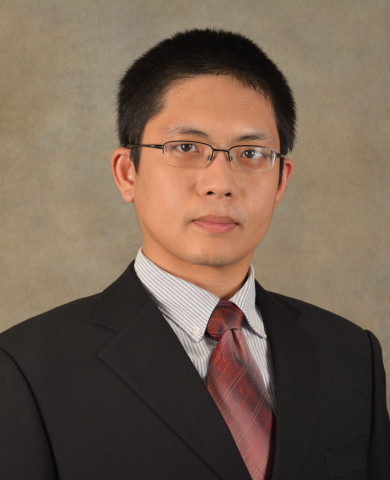
\includegraphics[width=28mm]{verticalYueHu.jpg}};
	\end{tikzpicture}
		
	\hypertarget{section}{%
\section{教育经历}\label{section}}

\begin{itemize}
\tightlist
\item
  美国爱荷华大学博士(政治学)\hfill 2018-05
\item
  美国南卡罗来纳大学硕士(政治学)\hfill 2013-03
\item
  加拿大里贾纳大学硕士(政治学)\hfill 2011-03
\item
  南开大学学士(国际关系)\hfill 2009-06
\end{itemize}

\hypertarget{section-1}{%
\section{工作经历}\label{section-1}}

\begin{itemize}
\tightlist
\item
  清华大学政治系助理教授\hfill 2019-01-02/今
\item
  美国爱荷华社会科学研究中心统计学顾问\hfill 2015-08/2018-05
\end{itemize}

\hypertarget{section-2}{%
\section{研究兴趣}\label{section-2}}

\begin{itemize}
\tightlist
\item
  \emph{比较政治}: 语言政治、经济与社会平等、政治传播。
\item
  \emph{方法论}: 政治实验、空间分析、文本分析、网络分析。
\item
  \emph{国际政治}: 公共外交、国际文化关系。
\end{itemize}

\hypertarget{section-3}{%
\section{发表}\label{section-3}}

\hypertarget{section-4}{%
\subsection{学术期刊}\label{section-4}}

Yue Hu. ``Are Informal Education Facilities Effective Means for
Generating Political Support? A Spatial Analysis''.
\emph{Social Science Quarterly} (2019). \url{https://rdcu.be/bj3NK}
(visited on 02/07/2019).

Vicki Hesli Claypool, William Reisinger, Marina Zaloznaya, Yue Hu, et
al. `\texttt{Tsar\ Putin\ and\ the}Corruption' Thorn in his Side: The
Demobilization of Votes in a Competitive Authoritarian Regime''.
\emph{Electoral Studies} 54 (2018), pp.~182--204.

``Economic Inequality and Class Consciousness''.
\emph{The Journal of Politics} 79.3 (2017), pp.~1079--1083.

Frederick Solt, Yue Hu, Kevan Hudson, Jungmin Song, et al. ``Economic
Inequality and Belief in Meritocracy in the United States''.
\emph{Research and Politics} 3.4 (2016), pp.~1-7.

Wenfang Tang, Yue Hu and Shuai Jin. ``Affirmative Inaction: Language
Education and Labor Mobility among China's Muslim Minorities''.
\emph{Chinese Sociological Review} 4.48 (2016), pp.~346-366.

Yue Hu. ``Institutional Difference and Cultural Difference: A
Comparative Study of Canadian and Chinese Cultural Diplomacy''.
\emph{Journal of American-East Asian Relations} 20.2-3 (2013),
pp.~256-268.

胡悦和朱毓朝:《`问题与主义' 导向之争:
西方比较政治学沿革及其借鉴意义》,载《天津社会科学》,2011年第3期,第46-50页。

程同顺和胡悦:《对外政策的文化道具:浅析文明冲突论的工具性》,载《学习论坛》2010年第26期,第33-7页。

胡悦:《从政治科学角度分析人民政协的政治定位》,载《天津市社会主义学院学报》
2009年第1期,第19-23页。

\hypertarget{section-5}{%
\subsection{研发软件}\label{section-5}}

Frederick Solt and Yue Hu. ``pewdata: Reproducible Retrieval of Pew
Research Center Datasets''. Available at The Comprehensive R Archive
Network (CRAN). 2016. \url{http://CRAN.R-project.org/package=pewdata}.

Frederick Solt and Yue Hu. ``dotwhisker: Dot-and-Whisker Plots of
Regression Results''. Available at The Comprehensive R Archive Network
(CRAN). 2015. \url{http://CRAN.R-project.org/package=dotwhisker}.

Frederick Solt and Yue Hu. ``interplot: Plot the Effects of Variables in
Interaction Terms''. Available at The Comprehensive R Archive Network
(CRAN). 2015. \url{http://CRAN.R-project.org/package=interplot}.

\hypertarget{section-6}{%
\subsection{期刊在审}\label{section-6}}

Yue Hu. ``Culture Marker vs.~Authority Marker: How Do Language Attitudes
Affect Political Trust?''

Yue Hu. ``Strategic Communication: Why the Chinese Government Engages in
Discourse about Democracy and Why It Matters''.

Amy Liu and Yue Hu. ``The Effects of Foreign Language Proficiency on
Public Attitudes: Evidence from the Chinese-Speaking World''.

\hypertarget{section-7}{%
\subsection{工作论文}\label{section-7}}

``Measure Political Desirability: An Experimental Method'' (with Wenfang
Tang).

``The Logic of Peaceful Rise: Revisiting the Power-Peace Relationship in
International Politics'' (with Ray Ou-Yang)

``The Popularity of Political Propaganda in Modern China: A Model of
Demands'' (with Zijie Shao).

\hypertarget{section-8}{%
\section{荣誉奖励}\label{section-8}}

\begin{itemize}
\tightlist
\item
  Ballard and Seashore 奖学金\hfill 2017
\item
  爱荷华大学Post-Comprehensive研究奖\hfill 2016
\item
  T. Anne Cleary国际博士论文奖学金 \hfill 2016
\end{itemize}

\hypertarget{section-9}{%
\section{专业训练}\label{section-9}}

\begin{itemize}
\tightlist
\item
  信息学辅修证书, 美国爱荷华大学\hfill 2016-12
\item
  实验研究方法, 新加坡国立大学 \hfill 2014-06/07
\end{itemize}

\hypertarget{section-10}{%
\section{特邀讲座}\label{section-10}}

\begin{itemize}
\tightlist
\item
  2018

  \begin{itemize}
  \tightlist
  \item
    ``Culture Marker vs.~Authority Marker: How Does Language Attitude
    Affect Political Trust?'' 中山大学,广州, 1月3日.
  \end{itemize}
\item
  2017

  \begin{itemize}
  \tightlist
  \item
    ``对社会经济不平等问题的实证研究:策略与方法.'' 南开大学,天津,
    6月25日.
  \end{itemize}
\end{itemize}

\hypertarget{section-11}{%
\section{会议活动}\label{section-11}}

\begin{itemize}
\tightlist
\item
  2018

  \begin{itemize}
  \tightlist
  \item
    ``Measuring the Influence of Language in Political Science
    Research.''

    \begin{itemize}
    \tightlist
    \item
      \footnotesize St.~Louis Area Methods Meeting (SLAMM), Ames, Iowa,
      Apr.~20.
    \end{itemize}
  \item
    ``Rebuilding the Tower of Babel? The Influence of Language Policy on
    Political Trust.''

    \begin{itemize}
    \tightlist
    \item
      \footnotesize Midwest Political Science Association (MPSA) Annual
      Convention, Chicago, Illinois, Apr.~5--8.
    \end{itemize}
  \end{itemize}
\item
  2017

  \begin{itemize}
  \tightlist
  \item
    ``Cultural Accent vs.~Authority Accent: How Does Language Attitude
    Affect Political Trust.''

    \begin{itemize}
    \tightlist
    \item
      \footnotesize 中国政治研究年会 (ACPS), 天津, 6月9--11日.
    \item
      \footnotesize 中国政治科学研究与方法工作坊, 上海, 7月8--9日.
    \item
      \footnotesize ``政治文化、心理与行为研究''工作坊, 南京,
      7月9--11日.
    \end{itemize}
  \item
    ``The Weight of History: Explaining the Anti-Japanese Sentiments in
    the Chinese Circle'' (with Amy Liu).

    \begin{itemize}
    \tightlist
    \item
      \footnotesize 美国中西部政治学会 (MPSA), 芝加哥,伊利诺伊,
      4月7--9日。
    \end{itemize}
  \item
    ``The Popularity of Political Propaganda in Modern China: A Model of
    Demands'' (with Zijie Shao).

    \begin{itemize}
    \tightlist
    \item
      \footnotesize 美国中西部政治学会 (MPSA), 芝加哥,伊利诺伊,
      4月7--9日。
    \end{itemize}
  \item
    ``The Logic of Peaceful Rise'' (with Ray Ou-Yang).

    \begin{itemize}
    \tightlist
    \item
      \footnotesize 美国中西部政治学会 (MPSA), 芝加哥,伊利诺伊,
      4月7--9日。
    \item
      \footnotesize 国际研究年会 (ISA), 巴尔的摩,马里兰, 二月22--25日。
    \end{itemize}
  \end{itemize}
\item
  2016

  \begin{itemize}
  \tightlist
  \item
    ``Measure Political Desirability: A List Experimental Method'' (with
    Wenfang Tang);
  \item
    ``Propaganda with Museums: A Spatial Analysis of Patriotic
    Educational Demonstration Bases in China.''

    \begin{itemize}
    \tightlist
    \item
      \footnotesize 中国政治研究年会 (ACPS), 蒙特利, 加利福尼亚,
      10月10--11日。
    \end{itemize}
  \item
    ``Value Promotion, Justification, or Mobilization? The Dynamic of
    the Discourse on Democracy in Modern China.''

    \begin{itemize}
    \tightlist
    \item
      \footnotesize 美国中西部政治学会 (MPSA), 芝加哥,伊利诺伊,
      4月7-10日。
    \end{itemize}
  \end{itemize}
\item
  2015

  \begin{itemize}
  \tightlist
  \item
    ``Affirmative Inaction: Education, Social Mobility, and Ethnic
    Inequality in China'' (with Wenfang Tang and Shuai Jin).
  \item
    ``Language and Political Trust.''

    \begin{itemize}
    \tightlist
    \item
      \footnotesize 美国中西部政治学会 (MPSA), 芝加哥,伊利诺伊,
      4月16--19日。
    \end{itemize}
  \end{itemize}
\item
  2013

  \begin{itemize}
  \tightlist
  \item
    ``Connecting Nationalism and Political Transition:A Study of
    Nationalist Influence on Political Transition based on the China
    Case.''

    \begin{itemize}
    \tightlist
    \item
      \footnotesize 南卡罗莱纳达研究生学会年会, 哥伦比亚,南卡罗来纳。
    \end{itemize}
  \end{itemize}
\item
  2012

  \begin{itemize}
  \tightlist
  \item
    ``Twofold-Affecting Model: A Cultural Pattern of Social Change from
    a Comparative Study between the China and Russia cases.''

    \begin{itemize}
    \tightlist
    \item
      \footnotesize 美国中国研究年会 (AACS), 奥特兰, 佐治亚,
      10月12-14日。
    \end{itemize}
  \end{itemize}
\end{itemize}

\hypertarget{section-12}{%
\section{科研项目}\label{section-12}}

\begin{itemize}
\tightlist
\item
  国家社科基金青年项目:基层党组织的政治生态评估体系与优化策略研究(项目编号17CZZ041)

  \begin{itemize}
  \tightlist
  \item
    项目参与人及研究方法指导 \hfill 2017/06-2020/06
  \end{itemize}
\end{itemize}

\hypertarget{section-13}{%
\section{教学经历}\label{section-13}}

\begin{itemize}
\tightlist
\item
  清华大学:

  \begin{itemize}
  \tightlist
  \item
    定量政治分析初步
  \item
    公共政策
  \item
    平等议题:理论与测量
  \end{itemize}
\item
  爱荷华大学:

  \begin{itemize}
  \tightlist
  \item
    政治学研究设计
  \item
    R语言与社会科学研究系列讲座
  \end{itemize}
\end{itemize}

\hypertarget{section-14}{%
\section{技能}\label{section-14}}

\begin{itemize}
\tightlist
\item
  分析与编程: R, Stata, Python, C++, Mathematica, NetLogo, JAGS, UCINET
\item
  应用: \LaTeX, Markdown, Git(GitHub)
\end{itemize}
	
			\end{document}